\documentclass[11pt,a4paper,landscape]{article}
\usepackage[margin=18mm]{geometry}
\usepackage{amsmath}
\usepackage{tikz}
\usetikzlibrary{arrows.meta,positioning,calc}
\pagestyle{empty}
\begin{document}
\begin{center}
{\Large\bfseries MATH6342 Linear Systems --- A1.1(ii)}\\[8pt]
$\displaystyle y+4\frac{d^2y}{dt^2}=2\frac{du}{dt}+7\int u\,dt$\\[7pt]
$\displaystyle y=\frac12\int u\,dt+\frac74\int\!\int\!\int u\,dt^3-\frac14\int\!\int y\,dt^2$
\end{center}
\vspace{12mm}
\begin{center}
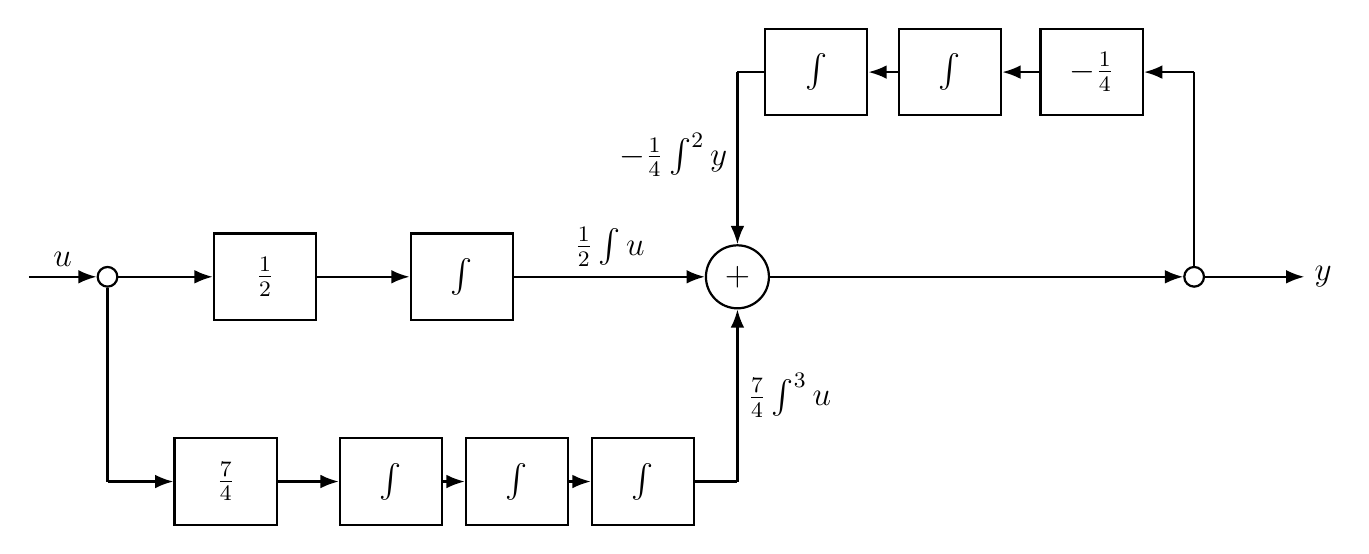
\begin{tikzpicture}[>=Latex, thick, every node/.style={font=\large},
  block/.style={draw,rectangle,minimum width=13mm,minimum height=11mm,inner sep=2pt},
  junction/.style={draw,circle,minimum size=8mm,inner sep=0pt},
  tap/.style={draw,circle,minimum size=2.5mm,inner sep=0pt,fill=white}]
% Main signal path
\coordinate (input) at (0,0);
\node[tap] (inputtap) at (1.0,0) {};
\node[block] (half) at (3.0,0) {$\frac12$};
\node[block] (intMain) at (5.5,0) {$\int$};
\node[junction] (sum) at (9,0) {$+$};
\node[tap] (outtap) at (14.8,0) {};
\draw[->] (input) -- node[above] {$u$} (inputtap);
\draw[->] (inputtap) -- (half);
\draw[->] (half) -- (intMain);
\draw[->] (intMain) -- node[above] {$\frac12\int u$} (sum);
\draw[->] (sum) -- (outtap);
\draw[->] (outtap) -- (16.2,0) node[right] {$y$};
% Lower input branch
\node[block] (gainSeven) at (2.5,-2.6) {$\frac74$};
\node[block] (int1) at (4.6,-2.6) {$\int$};
\node[block] (int2) at (6.2,-2.6) {$\int$};
\node[block] (int3) at (7.8,-2.6) {$\int$};
\draw[-] (inputtap) -- (1,-2.6);
\draw[->] (1,-2.6) -- (gainSeven);
\draw[->] (gainSeven) -- (int1);
\draw[->] (int1) -- (int2);
\draw[->] (int2) -- (int3);
\draw[-] (int3) -- (9,-2.6);
\draw[->] (9,-2.6) -- node[right,pos=.5] {$\frac74\int^3u$} (sum.south);
% Top feedback: flow from right to left
\node[block] (neg) at (13.5,2.6) {$-\frac14$};
\node[block] (feedbackInt1) at (11.7,2.6) {$\int$};
\node[block] (feedbackInt2) at (10.0,2.6) {$\int$};
\draw[-] (outtap) -- (14.8,2.6);
\draw[->] (14.8,2.6) -- (neg);
\draw[->] (neg) -- (feedbackInt1);
\draw[->] (feedbackInt1) -- (feedbackInt2);
\draw[-] (feedbackInt2) -- (9,2.6);
\draw[->] (9,2.6) -- node[left,pos=.48] {$-\frac14\int^2y$} (sum.north);
\end{tikzpicture}
\end{center}
\vspace{6mm}
\noindent\textbf{Lecture-note notation:} Rectangles denote amplifiers and integrators; small circles are taps; the $+$ circle is a summing junction. The upper branch feeds the output back into the sum. No differentiators appear. Integral formulas are understood with zero initial conditions.
\end{document}
